% This is "sig-alternate.tex" V2.1 April 2013
% This file should be compiled with V2.5 of "sig-alternate.cls" May 2012
%
% This example file demonstrates the use of the 'sig-alternate.cls'
% V2.5 LaTeX2e document class file. It is for those submitting
% articles to ACM Conference Proceedings WHO DO NOT WISH TO
% STRICTLY ADHERE TO THE SIGS (PUBS-BOARD-ENDORSED) STYLE.
% The 'sig-alternate.cls' file will produce a similar-looking,
% albeit, 'tighter' paper resulting in, invariably, fewer pages.
%
% ----------------------------------------------------------------------------------------------------------------
% This .tex file (and associated .cls V2.5) produces:
%       1) The Permission Statement
%       2) The Conference (location) Info information
%       3) The Copyright Line with ACM data
%       4) NO page numbers
%
% as against the acm_proc_article-sp.cls file which
% DOES NOT produce 1) thru' 3) above.
%
% Using 'sig-alternate.cls' you have control, however, from within
% the source .tex file, over both the CopyrightYear
% (defaulted to 200X) and the ACM Copyright Data
% (defaulted to X-XXXXX-XX-X/XX/XX).
% e.g.
% \CopyrightYear{2007} will cause 2007 to appear in the copyright line.
% \crdata{0-12345-67-8/90/12} will cause 0-12345-67-8/90/12 to appear in the copyright line.
%
% ---------------------------------------------------------------------------------------------------------------
% This .tex source is an example which *does* use
% the .bib file (from which the .bbl file % is produced).
% REMEMBER HOWEVER: After having produced the .bbl file,
% and prior to final submission, you *NEED* to 'insert'
% your .bbl file into your source .tex file so as to provide
% ONE 'self-contained' source file.
%
% ================= IF YOU HAVE QUESTIONS =======================
% Questions regarding the SIGS styles, SIGS policies and
% procedures, Conferences etc. should be sent to
% Adrienne Griscti (griscti@acm.org)
%
% Technical questions _only_ to
% Gerald Murray (murray@hq.acm.org)
% ===============================================================
%
% For tracking purposes - this is V2.0 - May 2012

\documentclass{sig-alternate-05-2015}

\usepackage{url}
\def\UrlBreaks{\do\/\do-}
\usepackage{breakurl}
\usepackage[breaklinks]{hyperref}
\usepackage{color}
\usepackage{subcaption}
\usepackage{cancel}
\usepackage{amsmath}
\usepackage{algorithm}
\usepackage[noend]{algpseudocode}
\captionsetup{compatibility=false}
\graphicspath{{./figures/}}
\newcommand{\annie}[1]{\emph{\color{red}(#1)}}


\makeatletter
\def\BState{\State\hskip-\ALG@thistlm}
\makeatother

\begin{document}

% Copyright
\setcopyright{acmcopyright}
%\setcopyright{acmlicensed}
%\setcopyright{rightsretained}
%\setcopyright{usgov}
%\setcopyright{usgovmixed}
%\setcopyright{cagov}
%\setcopyright{cagovmixed}


% DOI
%\doi{10.475/123_4}

% ISBN
%\isbn{123-4567-24-567/08/06}

%Conference
%\conferenceinfo{PLDI '13}{June 16--19, 2013, Seattle, WA, USA}

%\acmPrice{\$15.00}

%
% --- Author Metadata here ---
%\conferenceinfo{WOODSTOCK}{'97 El Paso, Texas USA}
%\CopyrightYear{2007} % Allows default copyright year (20XX) to be over-ridden - IF NEED BE.
%\crdata{0-12345-67-8/90/01}  % Allows default copyright data (0-89791-88-6/97/05) to be over-ridden - IF NEED BE.
% --- End of Author Metadata ---

\title{A First Look into Transnational Routing Detours}
%
% You need the command \numberofauthors to handle the 'placement
% and alignment' of the authors beneath the title.
%
% For aesthetic reasons, we recommend 'three authors at a time'
% i.e. three 'name/affiliation blocks' be placed beneath the title.
%
% NOTE: You are NOT restricted in how many 'rows' of
% "name/affiliations" may appear. We just ask that you restrict
% the number of 'columns' to three.
%
% Because of the available 'opening page real-estate'
% we ask you to refrain from putting more than six authors
% (two rows with three columns) beneath the article title.
% More than six makes the first-page appear very cluttered indeed.
%
% Use the \alignauthor commands to handle the names
% and affiliations for an 'aesthetic maximum' of six authors.
% Add names, affiliations, addresses for
% the seventh etc. author(s) as the argument for the
% \additionalauthors command.
% These 'additional authors' will be output/set for you
% without further effort on your part as the last section in
% the body of your article BEFORE References or any Appendices.

\numberofauthors{4} %  in this sample file, there are a *total*
% of EIGHT authors. SIX appear on the 'first-page' (for formatting
% reasons) and the remaining two appear in the \additionalauthors section.
%
\author{
% You can go ahead and credit any number of authors here,
% e.g. one 'row of three' or two rows (consisting of one row of three
% and a second row of one, two or three).
%
% The command \alignauthor (no curly braces needed) should
% precede each author name, affiliation/snail-mail address and
% e-mail address. Additionally, tag each line of
% affiliation/address with \affaddr, and tag the
% e-mail address with \email.
%
% 1st. author
%\alignauthor
%Anne Edmundson\\
%       \affaddr{Princeton University}\\
%       \email{annee@cs.princeton.edu}
% 2nd. author
%\alignauthor
%Roya Ensafi\\
%       \affaddr{Princeton University}\\
%       \email{ensafi@cs.princeton.edu}
%\and % use '\and' if you need 'another row' of author names
% 3rd. author
%\alignauthor Jennifer Rexford\\
%       \affaddr{Princeton University}\\
%       \email{jrex@cs.princeton.edu}
% 4th. author
%\alignauthor Nick Feamster\\
%       \affaddr{Princeton University}\\
%       \email{feamster@cs.princeton.edu}
}

\date{}

\maketitle
\begin{abstract}
An increasing number of countries are passing laws that facilitate the
mass surveillance of their citizens. In response, governments and
citizens are increasingly paying attention to the countries that their
Internet traffic traverses. In some cases, countries are taking extreme
steps, such as building new IXPs and encouraging local interconnection
to keep local traffic local. We find that although many of these efforts
are extensive, they are often futile, due to the inherent lack of
hosting and route diversity for many popular sites. First, we characterize 
transnational routing detours by measuring the country-level paths to 
popular domains.  Then, we investigate how
the use of overlay network relays and the DNS open resolver
infrastructure can prevent traffic from traversing certain jurisdictions. 
We find that current traffic is traversing known surveillance states, but 
also show that there are tools that can be used for country avoidance. Our 
results show that 84\% of paths originating in Brazil traverse the United States, 
but when relays are used for country avoidance, only 37\% of Brazilian paths 
traverse the United States.  Unfortunately, we also find that 
some of the more prominent surveillance states are also some of the least avoidable 
countries.
\end{abstract}


%
% The code below should be generated by the tool at
% http://dl.acm.org/ccs.cfm
% Please copy and paste the code instead of the example below. 
%
\begin{CCSXML}
<ccs2012>
<concept>
<concept_id>10002978.10003014</concept_id>
<concept_desc>Security and privacy~Network security</concept_desc>
<concept_significance>300</concept_significance>
</concept>
</ccs2012>
\end{CCSXML}

\ccsdesc[300]{Security and privacy~Network security}
%
% End generated code
%

%
%  Use this command to print the description
%
\printccsdesc

% We no longer use \terms command
%\terms{Theory}

%\keywords{ACM proceedings; \LaTeX; text tagging}

\section{Introduction}
\label{intro}

There are no restrictions on which national jurisdictions BGP paths must or must not cross.  There is also no way for an Internet user to know or decide which countries her Internet traffic is transitting.  Internet routing is usually studied at the AS (Autonomous System) level - not the nation-state level.  An AS typically controls traffic as it transits it's internal network and then defines policies for filtering, monitoring, and routing traffic to the next AS.  It is becoming increasingly common for governments to require certain actions of ASes, such as enabling wiretapping or performing censorship.  Once Internet traffic enters a country, it is subject to that country's requirements, and subsequently the corresponding ASes' actions.  More and more countries are either trying or have already passed laws that allow for mass surveillance on their citizens~\cite{france_surveillance, netherlands_surveillance, kazak_surveillance}.  Recently, the Investigatory Powers Bill (IP Bill) in the UK, if passed, will require ISPs to store citizens' browsing history for a year, and allow intelligence agencies to collect bulk data on their citizens~\cite{uk_bill}.

Currently, governments are becoming more suspicious about where their citizens' traffic is going, and are facing the challenge of controlling which countries transit the traffic.  Governments and users have been motivated more than ever since the Snowden revelations to avoid countries known for surveillance practices, specifically the United States~\cite{russia_secure_internet, routing_errors, dte}.  More recently, the Safe Harbour agreement, an agreement that allows the free flow of data between the US and the EU, was struck down because it would give the NSA access to EU citizens' personal data~\cite{safe_harbour_illegal, safe_harbour_undecided}.

In response to the Snowden revelations, Brazil has taken great measures to avoid Internet traffic from being wiretapped by the NSA~\cite{brazil_history, brazil_break_from_US, brazil_conference, brazil_conference2, brazil_human_rights}.  Some of the actions that have been taken to avoid NSA surveillance include: building a 3,500 mile long fiber-optic cable from Fortaleza to Portugal (with no use of American vendors), pressing companies such as Google, Facebook, and Twitter (among others) to store data locally, switching its dominant email system (Microsoft Outlook) to a state-developed system called Expresso~\cite{brazil_cable, brazil_us_companies}.  In other efforts, Brazil has been building Internet eXchange Points, which help grow Internet connectivity and performance~\cite{brazil_IXP1, brazil_IXP2}; it also allows them to increase their connectivity with many other countries.  Brazil now has the largest national ecosystem of public Internet eXchange points in the world~\cite{brazil_ixp_ecosystem}.  It has also been shown that over the past few years, the number of ASes in Brazil that are connected internationally have grown significantly~\cite{brazil_international_ases}.  The case of Brazil shows that countries, governments, and Internet users are motivated to avoid surveillance conducted by other countries.

Determining which countries transit Internet traffic, which countries host the only server for a given domain, and which countries are avoidable for a given domain are challenging problems.  The first challeng arises from determining the country-level path that traffic takes; paths can be collected from either the data-plane - IP-level paths - or the control-plane - AS-level paths.  Our work uses the data-plane to analyze traffic paths; in order to determine which countries are on the path, the IP-level path must be mapped to a country-level path.  This is challenging because there is no ground truth for geolocation data; there is no guarantee of accuracy or completeness.  To address this challenge, we use different geolocation tools to increase our confidence in the country-level paths we collect.  More challenges arise in determining how to avoid countries; websites are complex and can fetch data from multiple third parties, which are likely located in different geographic locations, and therefore cross different countries' borders.  The increased usage of anycast IP complicates country avoidance because it gives clients less information about the location of the server from which they are accessing content.  

In this paper, we first shed light on how much traffic is currently transiting countries known for surveillance, with a focus on the US.  Despite the measures taken by different countries to avoid the US, we still see Internet traffic that transits the US.  We conduct a measurement study that helps quantify the existing possibilities for state-sponsored surveillance.  We take Brazil as a case study, and analyze the country-level paths from machines in Brazil to the Brazil Alexa Top 100 domains.  Knowing that Brazil has taken actions to avoid traffic transitting the US, we measure how much traffic is solely transitting the US, and how much traffic is destined for the US.  These are two distinct scenarios.  If the US is solely a country on the path (and not the end point), then there is the possibility for avoiding the US.  If the domain is solely hosted in the US, and therefore destined for the US, then the US cannot be avoided for the given domain.  Using RIPE Atlas probes and the Digital Envoy geolocation service, we find that out of 36,833 traffic paths originating in Brazil to the Brazilian Alexa Top 100 domains, 2,699 are solely transitting the US and the US is the destination for 28,196 of them (this does not necessarily mean that the US is the only possible destination, but it is the destination for Brazilian Internet users)~\cite{ripe_atlas, digital_envoy}.  

Next, we present and implement a new system for surveillance circumvention for Internet users, which finally gives the users some control over where their traffic is flowing.  Because popular web companies are opening or expanding their datacenters in Europe, there are more possible paths to get data~\cite{eu_datacenters}.  It is possible that a path from a client in Brazil to a datacenter in Europe does not pass through any country known for surveillance, but may be a longer path than the best path to a datacenter in the US, as shown in Figure~\ref{fig:intro}.  Our system leverages a geographically diverse set of relay machines that act as proxies to access data from servers located in different geographic regions.  A client will first query an oracle for the best relay to use in order to avoid a given country.  Then the oracle will respond with the IP address of the best relay, which the client will then send it's request to.  The relay will fetch the data from the domain's closest server and return the data to the client. \annie{Add a couple highlights of the results/evaluation section when we get there.}

\begin{figure}
\centering
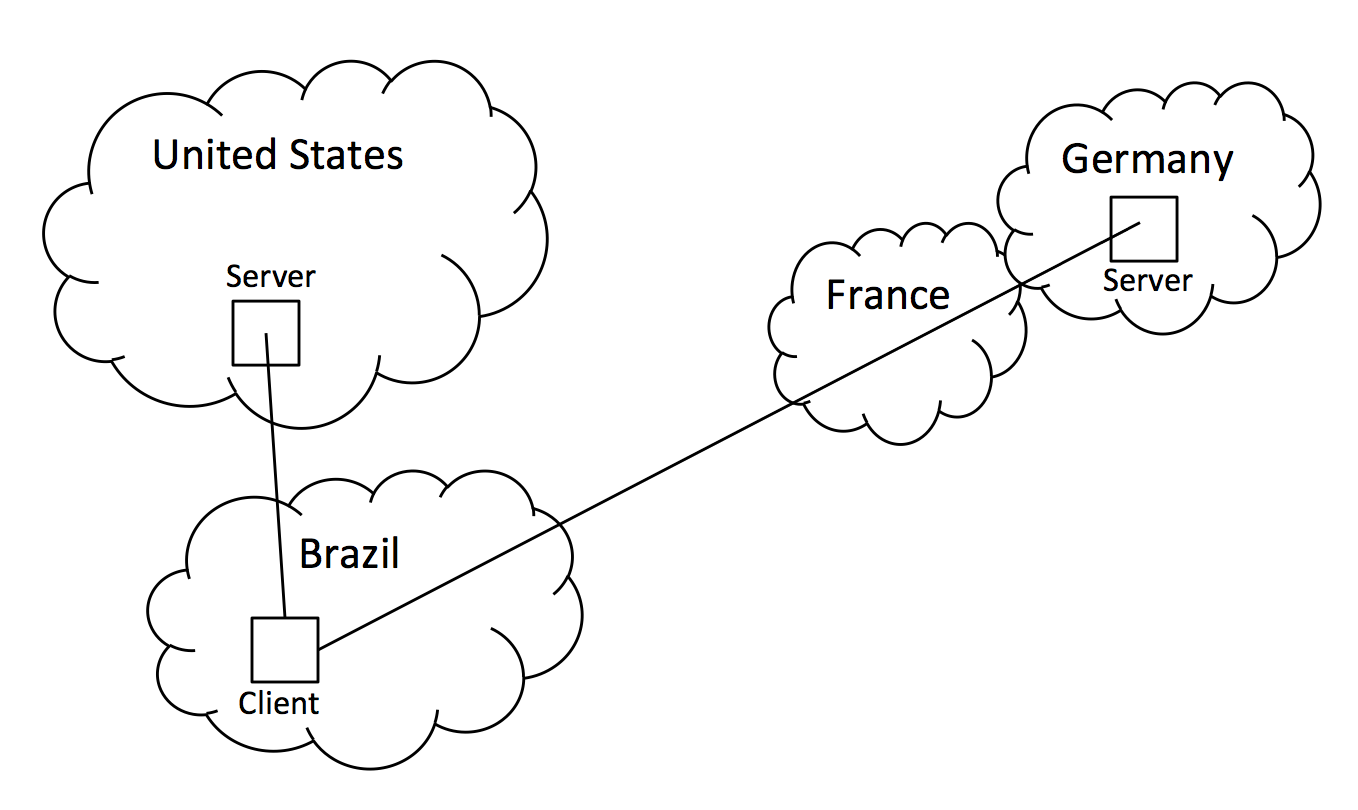
\includegraphics[width=.5\textwidth]{intro_fig}
\caption{A shorter path to a server in a country known for surveillance (U.S.), and a longer path to a georeplicated server in Germany.  The longer path may be more preferred by the client because it doesn't traverse a country with known surveillance practices.}
\label{fig:intro}
\end{figure}

This paper is organized as follows.  In the next section, we describe our research goals, and the challenges in achieving them.  In Section~\ref{datasets} we discuss how and where we collected our data.  We point out the advantages and disadvantages of existing datasets, and justify our decision.  In Section \ref{measure}, we design and execute a measurement study on the country-level paths of Brazil's Internet.  We describe our methodology, as well as results that show which countries Brazil's Internet traffic is traversing.  Next, Section \ref{architecture} introduces SYSTEM, which allows Internet users, ISPs, and Internet services to avoid specified countries, and therefore circumvent surveillance.  Then we explain our implementation of SYSTEM in Section \ref{implementation}.  In Section \ref{evaluation}, we evaluate our system and proposed methods for how well they avoid any given country.  We discuss how our system differs from others and uniquely suits the purpose of country avoidance in Section \ref{discussion}, we review related work in Section \ref{related}, and conclude in Section \ref{conclusion}.

\section{State of Surveillance}
\label{surv}
We focused our study on five different countries, and for each, we actively measured and analyzed traffic that originated there.  These five countries were chosen for specific reasons and we present them here.  We also discuss countries that currently conduct surveillance; this exploration is not exhaustive, but highlights countries that are passing new surveillance laws and countries that have strict surveillance practices already.   

\subsection{Studied Countries}
We selected Brazil, Netherlands, Kenya, India, and the United States for the following reasons.

\paragraph{Brazil.} It has been widely publicized that Brazil is actively trying to avoid having their traffic transit the United States.  They have been building IXPs, deploying underwater cables to Europe, and pressuring large U.S. companies to host content within Brazil~\cite{brazil_history, brazil_break_from_US, brazil_conference,
  brazil_conference2, brazil_human_rights, brazil_cable, brazil_us_companies, brazil_IXP1}.  This effort to avoid traffic transitting a specific country led us to investigate whether their efforts have been successful or not.

\paragraph{Netherlands.}  We selected to study the Netherlands for three reasons: 1) the Netherlands is beginning to emerge as a site where servers are located for cloud services, such as Akamai, 2) the Netherlands is where a large IXP is located (AMS-IX), and 3) they are drafting a mass surveillance law~\cite{netherlands_surveillance}. Analyzing the Netherlands will allow us to see what effect AMS-IX and the emergence of cloud service hosting has on their traffic.

\paragraph{Kenya.} Prior research on the interconnectivity of Africa~\cite{gupta2014peering, fanou2015diversity} led us to explore the characterization an African country's interconnectivity.  We chose Kenya for several reasons: 1) it has more than one IXP, 2) it has high Internet access and usage (for the East African region), and 3) it is a location with many submarine cable landing points~\cite{kenya_nigeria, teams}.

\paragraph{India.}  India has one of the highest number of Internet users in Asia, second only to China, which has already been well-studied~\cite{tsui2003panopticon, wang2010discourse}.  With such a high number of Internet users, and presumably a large amount of Internet traffic, we study India to see where this traffic is going.

\paragraph{United States.}  We chose to study the United States because of how inexpensive it is to host domains there, as well as the prevalence of Internet and technology companies located there.

\subsection{Surveillance States}

%Some countries have created agreements on data sharing, while others want to control their citizens' online presence.  
When analyzing which countries Internet traffic traverse, special attention should be given to countries that may be unfavorable because of their surveillance laws.  Some of the countries that are currently conducting surveillance are the ``Five Eyes'' ~\cite{lander2004international, eyeswideopen} (the United States, Canada, United Kingdom, New Zealand, and Australia), as well as France, Germany, Poland, Hungary, Russia, Ukraine, Belarus, Kyrgyzstan, and Kazakhstan.  

\paragraph{Five Eyes.} The ``Five Eyes'' participants are the United States National Security Agency (NSA), the United Kingdom's Government Communications Headquarters (GCHQ), Canada's Communications Security Establishment Canada (CSEC), the Australian Signals Directorate (ASD), and New Zealand's Government Communications Security Bureau (GCSB)~\cite{eyeswideopen}.  According to the original agreement, the agencies can: 1) collect traffic; 2) acquire communications documents and equipment; 3) conduct traffic analysis; 4) conduct cryptanalysis; 5) decrypt and translate; 6) acquire information about communications organizations, procedures, practices, and equipment.  The agreement also implies that all five countries will share all intercepted material by default.  The agencies work so closely that the facilities are often jointly staffed by members of the different agencies, and it was reported ``that SIGINT customers in both capitals seldom know which country generated either the access or the product itself.''~\cite{lander2004international}.

\begin{table}[t!]
\centering
\begin{small}
\resizebox{\columnwidth}{!}{%
\begin{tabular}{|p{2cm}|p{1.6cm}p{1.6cm}p{1.6cm}p{1.6cm}|}
\hline
 & Collecting Metadata (Phone, Internet) & Requiring ISPs to Participate & No Need for Court Order & Targeted Surveillance \\
\hline
France            & \checkmark~\cite{francesurv, francesurv2} & \checkmark~\cite{francesurv} &  & \\ 
Germany           & \checkmark~\cite{germansurv}   &             &             &                  \\ 
UA Emirates & & & & \checkmark~\cite{uae_surv} \\
Bahrain & & & & \checkmark~\cite{bahrain_surv} \\
Australia & \checkmark~\cite{eyeswideopen} & &  &\\
New Zealand & \checkmark~\cite{eyeswideopen} & &  & \\
Canada & \checkmark~\cite{eyeswideopen} & & & \\
United States & \checkmark~\cite{eyeswideopen} & & & \\
Great Britain & \checkmark~\cite{eyeswideopen} & & & \\
Poland            & \checkmark~\cite{francesurv2}      &         &  \checkmark~\cite{francesurv2}      &      \\ 
Hungary            & \checkmark~\cite{francesurv2}        &             & \checkmark~\cite{francesurv2} & \\ 
Ukraine            & \checkmark~\cite{francesurv2}    & \checkmark~\cite{russiasurv, russiasurv2}    & &  \\ 
Belarus            & \checkmark~\cite{francesurv2}    & \checkmark~\cite{russiasurv, russiasurv2}    & &  \\ 
Kyrgyzstan            & \checkmark~\cite{francesurv2}    & \checkmark~\cite{russiasurv, russiasurv2}    & &  \\ 
Kazakhstan            & \checkmark~\cite{francesurv2}    & \checkmark~\cite{russiasurv, russiasurv2}    & &  \\ 
Russia            & \checkmark~\cite{francesurv2}    & \checkmark~\cite{russiasurv, russiasurv2}    & &  \\ \hline
%....              &      &        &   \\    \hline
\end{tabular}
}
\end{small}
\caption{Some countries that actively conduct surveillance.}
\label{surv_table}
\end{table}

A number of other countries are passing laws to facilitate mass surveillance.  These laws have differing levels of intensity, which can be seen in Table \ref{surv_table}; the countries with the least intense surveillance laws are listed at the top of the table, and those with the more intense laws are listed at the bottom.  These countries, along with the ``Five Eyes'' participants should be flagged when characterizing transnational detours in the following section.

%\paragraph{France.} France recently passed a new surveillance law that authorizes the government closely monitor the mobile phone and Internet communications of French citizens.  Additionally, the law requires ISPs to install ``black boxes'' that are designed to collect and analyze metadata on the Internet usage of millions of people.  The law allows surveillance without much oversight and the conditions under which the law's powers can be used are vague~\cite{francesurv}. The French Parliament has also made it easier for the government to access encrypted data for criminal investigations by enhancing penalties against companies that refuse to cooperate~\cite{francesurv2}.

%\paragraph{Germany.} A new data retention law was recently passed in Germany that will allow law enforcement agencies to access metadata of phone calls and Internet connections~\cite{germansurv}.  Prior to the bill, telecom providers only retained data for business purposes, but the bill will modify the German Telecommunications Act and require telecom providers to retain traffic data on phone calls and Internet connections.  The data collected includes IP addresses of users as well as the date and time of Internet connections.

%\paragraph{Poland.}  Poland now has stricter surveillance laws by ammending the Police Act.  This gives Polish authorities access to metadata without court approval~\cite{francesurv2}.

%\paragraph{Hungary.}  Hungary has pushed surveillance even further by proposing a new bill that makes it a crime for service providers to use encryption-based application or software.  It also forces ISPs to build back doors that give the government access to data.  Under the bill, ISPs are required to collect metadata on anyone who uses encryption, and it criminalizes the refusal of companies to give collected data to the government~\cite{francesurv2}.

%\paragraph{Russia.} Russia has had a surveillance infrastructure for years: SORM (System of Operative-Investigative Measures).  SORM involves a series of black boxes that ISPs must install; the providers are required to pay for the SORM equipment and installation and they are denied access to the box~\cite{russiasurv}.  If an ISP fails to cooperate, it is fined, and if the violation persists, then its license may be revoked.  Former Soviet Republics have followed in Russia's footsteps: Belarus, Ukraine, and Kyrgyzstan have adopted national interception systems modeled after SORM~\cite{russiasurv}.  Many popular sites, such as Facebook, Google, and Twitter are not hosted in Russia, which challenges surveillance.  In the past year, Russia has passed a data localization law.  This law states that any company that collects personal information from Russian users must stor their data on servers within the country - the main targets of the law were Facebook, Google, and Twitter~\cite{russiasurv2}. 

\section{Characterizing Transnational Detours}
\label{datasets}
In this section, we introduce our measurement methods, challenges in conducting the measurements, and our findings on which countries current traffic traverses.

\begin{figure*}[t]
\centering
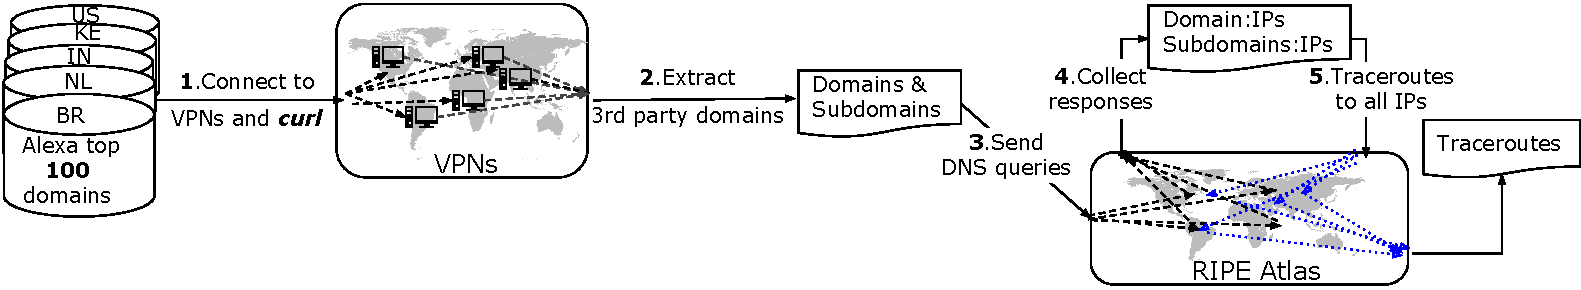
\includegraphics[width=.9\textwidth]{Current-Traffic_fig}
\caption{The measurement pipeline to study current traffic routes.}
\label{fig:pipeline1}
\end{figure*}

\begin{figure}[t]
\centering
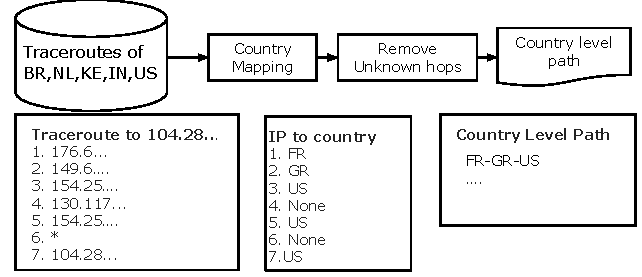
\includegraphics[width=.5\textwidth]{Analysis-Pipeline1}
\caption{The measurement pipeline to analyze traceroutes.}
\label{fig:analysis_pipeline}
\end{figure}

\subsection{Measurement Pipeline}
\label{pipeline}
We use the data plane to measure traffic paths; we analyze the reported hops of traceroute measurements to find which countries are on the path from a client in a particular country to a popular domain.  The reverse path is just as important as the forward path, and often the reverse path is different from the forward path; we measure how symmetric the forward and reverse paths are the country-level in Section \ref{path_sym}, and also explain how the exclusion of the reverse path provides a lower bound on the number of countries that traffic traverses.  Using traceroutes to measure transnational detours is new; prior work used BGP routing tables to \textit{infer} country-level paths~\cite{karlin2009nation}.  Because we conduct active measurements, which are limited by our resources, we make a tradeoff and study five countries, as opposed to all countries' Internet paths.  Figure \ref{fig:pipeline1} shows the steps taken for this measurement; first we identify a set of popular domains, then we use RIPE Atlas probes to query DNS with these domains, and traceroute to the DNS responses.  The measurements were conducted on January 31st, 2016.  Our analysis involves the steps seen in Figure \ref{fig:analysis_pipeline}; we map traceroutes to country-level paths.

\subsubsection{Resource Limitations}
\label{resource_limits}
To our knowledge, the publicly available traceroute datasets suitable for our goal are from iPlane~\cite{madhyastha2006iplane} and CAIDA (Center for Applied Internet Data Analysis)~\cite{caida}.  The iPlane project uses PlanetLab~\cite{planetlab} nodes to run traceroutes to all unique AS-level paths in the BGP routing table.  This project also has historical data as far back as 2006.  Unfortunately, because iPlane uses PlanetLab nodes, which have been shown to mostly use the Global Research and Education Network (GREN), the traceroutes from PlanetLab nodes will not be representative of typical Internet users' traffic paths~\cite{banerjee2004interdomain}.  The other publicly available dataset, from CAIDA, ran traceroutes from different vantage points around the world, but to randomized destination IP addresses that cover all /24s.  This is also not sufficient for what we wanted to measure because a typical Internet user is going to access a domain that will be locally resolved; the user will not input a specific IP address in their browser.  

We chose to run active measurements that would be most representative of an Internet user.  We chose to run DNS and traceroute measurements from RIPE Atlas probes, which are hosted all around the world and in many different settings, including home networks~\cite{ripe_atlas}.  RIPE Atlas probes can use the local DNS resolver, which would give us the best estimate of the traceroute destination.

Despite the options RIPE Atlas provides, there were still restrictions that made measurements challenging.  To conduct any measurement on a RIPE Atlas probe, it costs a certain amount of credits, and we were therefore restricted by the number of credits we had.  Additionally, RIPE Atlas imposes rate limits on the number of concurrent measurements and the number of credits that an individual user can spend per day.  We address these challenges in two ways: 1) we reduce the number of necessary measurements we must run on RIPE Atlas probes by conducting traceroute measurements to a single IP address in each /24 (as opposed to all IP address returned by DNS) because all IP addresses in a /24 belong to the same AS, and should therefore be located in the same geographic area; 2) use a different method---VPN connections---to get a vantage point within a foreign country, which is still representative of an Internet user in that country.

\subsubsection{Path Asymmetry}
\label{path_sym}
Previous work has shown that paths are not symmetric most of the time---the forward path from point A to point B does not match the reverse path from point B to point A~\cite{he2005routing}.  Most work on path asymmetry has been done at the AS level, but not at the country level.  Our measurement methods only take the forward path (from client to domain or relay) into account, and not the path from the domain or relay to the client.  

We conducted a study to measure path asymmetry at the country granularity; if country-level paths are symmetric, then the results of our measurements would be representative of the forward {\it and} reverse paths, but if the country-level paths are asymmetric, then our measurement results only provide a lowerbound on the number of countries that could potentially conduct surveillance.  Using 100 RIPE Atlas probes located around the world, and 8 Amazon EC2 instances, we ran traceroute measurements from every probe to every EC2 instance and from every EC2 instance to every probe.  After geolocating the IPs to countries, we analyzed the paths for symmetry.  First, we compared the set of countries on the forward path to the set of countries on the reverse path; this yielded about 30\% symmetry.  What we wanted to know is whether or not the reverse path has more countries on it than the forward path.  We measured how many reverse paths were a subset of the respective forward path; this was the case for 55\% of the paths.  

The results of this measurement are not convincing enough to state that country-level paths are symmetric, and therefore our measurements and results represent a lowerbound on the number of countries that transit traffic; our results are a lowerbound on how many unfavorable countries transit a client's traffic.

\subsubsection{Traceroute Origination and Destination Selection}
As discussed above, we used RIPE Atlas probes in each of the five countries we studied.  Each of these countries had varying amounts of probes hosted in the country, ranging from about 75 probes to many hundreds.  Because of the resource restrictions, we could not use all probes in each of the countries.  We selected the set of probes that had unique ASes in the country to get the widest representation of origination (starting) points.

For destinations, we used the Alexa Top 100 domains in each of the respective countries, as well as the 3rd party domains that are requested as part of an original web request.  To obtain these 3rd party domains we {\tt curl} (fetch) each of the Top 100 domains, but we must do so from within the country we are studying.  There is no current functionality to {\tt curl} from RIPE Atlas probes, so we establish a VPN connection within each of these countries to {\tt curl} each domain and extract the 3rd party domains; we {\tt curl} from the client's location in case web sites are customizing content based on the region of the client.

\subsubsection{Country Mapping}
\label{c_map}
Geolocation services and tools have been studied and proposed, and continue to be a growing research area.  Because that is not the primary focus of our work, we use MaxMind's geolocation service to map IP addresses to their respective countries~\cite{maxmind}.   Our study requires country-level paths, which is a coarser granularity than either city granularity or latitude-longitude granularity.  Previous work has studied the inaccuracy of geolocation services, but the evaluation was at the latitude-longitude granularity~\cite{huffaker2011geocompare}; we observe less inaccuracy at the country-level.  To address the incompleteness of the data, we cleaned up our IP to country mapping by removing all IP addresses that resulted in a `None' response when querying MaxMind, which causes our results to provide a conservative estimate of the number of countries that traffic passes through. It is important to note that removing `None' responses will \textit{always} produce a conservative estimate, and therefore we are \textit{always} underestimating the amount of potential surveillance.  An example of this can be seen in Figure \ref{fig:analysis_pipeline}.  This method provides a lower bound on the number of countries that are included on the path, and therefore a lower bound on the countries that can conduct surveillance.  

\subsection{Results}

%%%% ADD THIS TO datasets.tex
\newcolumntype{d}[1]{D{.}{.}{#1}}
\newcommand{\headrow}[1]{\multicolumn{1}{c}{\adjustbox{angle=45,lap=\width-0.5em}{#1}}}
\newcolumntype{P}[1]{>{\raggedright\arraybackslash}p{#1}}
\newcommand{\ra}[1]{\renewcommand{\arraystretch}{#1}}
\begin{table}[t]
\centering
\ra{1.2}
\resizebox{\columnwidth}{!}{%
\begin{tabular}{@{}ld{3.2}d{3.2}d{3.2}d{3.2}d{3.2}@{}}
%\multicolumn{1}{l}{}    & \headrow{Host} & \headrow{Transit} & \headrow{Host} & \headrow{Transit} &\headrow{Host} &\headrow{Transit} &\headrow{Host}   &\headrow{Transit} &\headrow{Host}  &\headrow{Transit} \\

\textit{Country}    & \headrow{Brazil}  & \headrow{Netherlands}   & \headrow{India} & \headrow{Kenya} & \headrow{United States}\\
\toprule
Brazil             &.169    &-     &-    & -  & - \\ \midrule
Canada             &.001    &.007     &.015      &.006       & -  \\
United States      &\cellcolor[HTML]{F7BE81}.774    &\cellcolor[HTML]{F7BE81}.454      &\cellcolor[HTML]{F7BE81}.629      &\cellcolor[HTML]{F7BE81}.443        &\cellcolor[HTML]{F7BE81}.969    \\ \midrule
France             &.001    &.022      &.009      &.023       &.001 \\
Germany            &.002    &.013      &.014      &.028       &.001  \\
Great Britain      &-  &.019     &.021     &.032       &.002 \\
Ireland            &.016    &.064      &.027       &.108       &.001   \\
Netherlands        &.013    &\cellcolor[HTML]{F7BE81}.392      &.101      &\cellcolor[HTML]{F7BE81}.200      &.024  \\
Spain              &.001    &-     & -    &  -     &-    \\ \midrule
Kenya              &-        &  -    & -    &.022        &-  \\
Mauritius          &  -      & -    & -   &.004       & -  \\
South Africa       & -       & -     & -  &.021       &-  \\ \midrule
United Arab Emirates & -     & -     & -   &.011        &-  \\
India              &  -      & -     &.053    &.002        &-  \\
Singapore          & -       &.002     &\cellcolor[HTML]{F7BE81}.103      &.027       & - \\\hline
\end{tabular}
}
\caption{Fraction of paths that end in each country in default routes.}
\label{tab:host}
\end{table}

\begin{table}[t]
\centering
\ra{1.2}
\resizebox{\columnwidth}{!}{%
\begin{tabular}{@{}ld{3.2}d{3.2}d{3.2}d{3.2}d{3.2}@{}}
%\multicolumn{1}{l}{}    & \headrow{Host} & \headrow{Transit} & \headrow{Host} & \headrow{Transit} &\headrow{Host} &\headrow{Transit} &\headrow{Host}   &\headrow{Transit} &\headrow{Host}  &\headrow{Transit} \\

\textit{Country}    & \headrow{Brazil}  & \headrow{Netherlands}   & \headrow{India} & \headrow{Kenya} & \headrow{United States}\\ \toprule
Brazil              &1.00       & -   & -     & -     & -\\ \midrule
Canada                &.013       &.007     &.016       &.008      &.081 \\
United States        &\cellcolor[HTML]{F7BE81}.844        &\cellcolor[HTML]{F7BE81}.583     &\cellcolor[HTML]{F7BE81}.715      &\cellcolor[HTML]{F7BE81}.616       &\cellcolor[HTML]{F7BE81}1.00 \\ \midrule
France                 &.059     &.102      &.104       &.221      &.104 \\
Germany                 &.005       &.050    &.032      &.048      &.008 \\
Great Britain                &.024       &\cellcolor[HTML]{F7BE81}.140     &\cellcolor[HTML]{F7BE81}.204      &\cellcolor[HTML]{F7BE81}.500      &.006 \\
Ireland                &.028       &.106      &.031     &.133      &.006 \\
Netherlands                 &.019        &1.00      &.121      &\cellcolor[HTML]{F7BE81}.253      &.031 \\\hline
Spain                  &.176       &.004     & -     & -      &- \\ \midrule
Kenya                 & -       &-    & -      &1.00      &- \\\hline
Mauritius                  & -       & -     & -      &\cellcolor[HTML]{F7BE81}.322       &- \\
South Africa                 &-        & -    & -     &\cellcolor[HTML]{F7BE81}.334       &- \\ \midrule
United Arab Emirates                  &.00003        & -    & -     &.152       &- \\
India               &  -    &.0007    &1.00     &.058     &.0005 \\
Singapore                 &.0009        &.002     &\cellcolor[HTML]{F7BE81}.270       &.040       &.003 \\ \midrule
\end{tabular}
}
\caption{Fraction of paths that each country transits in default routes.}
\label{tab:transit}
\end{table}

Table \ref{tab:host} shows the five studied countries along the top of the table, and the countries that host their traffic along the Y axis.  For example, the United States is the endpoint of 84\% of the paths that originate in Brazil.  A ``-'' represents the case where no traffic ended in that country.  For example, no Brazilian paths ended in South Africa. Table \ref{tab:transit} shows the fraction of paths that transit certain countries (along the Y axis).

\begin{finding}[Hosting Diversity]
About half of the top domains in each of the five countries studied are hosted in a single country.
\end{finding}
First we analyzed hosting diversity; this shows us how many unique countries in which a domain is hosted---the more countries that a domain is hosted in creates a greater chance that the content is replicated in a favorable country, and could potentially allow a client to circumvent an unfavorable country.  We queried DNS from 26 vantage points around the world, which are shown in Figure \ref{fig:world}; we chose this set of locations because they are geographically diverse.  Figure~\ref{fig:host_diversity} shows two common hosting cases: 1) CDNs, and 2) a single hosting country.  This shows that many domains are hosted in a single unique country, which leads us to our next analysis---where are these domains hosted, and which countries are traversed on the way to reach these locations.

\begin{figure}[t]
\centering
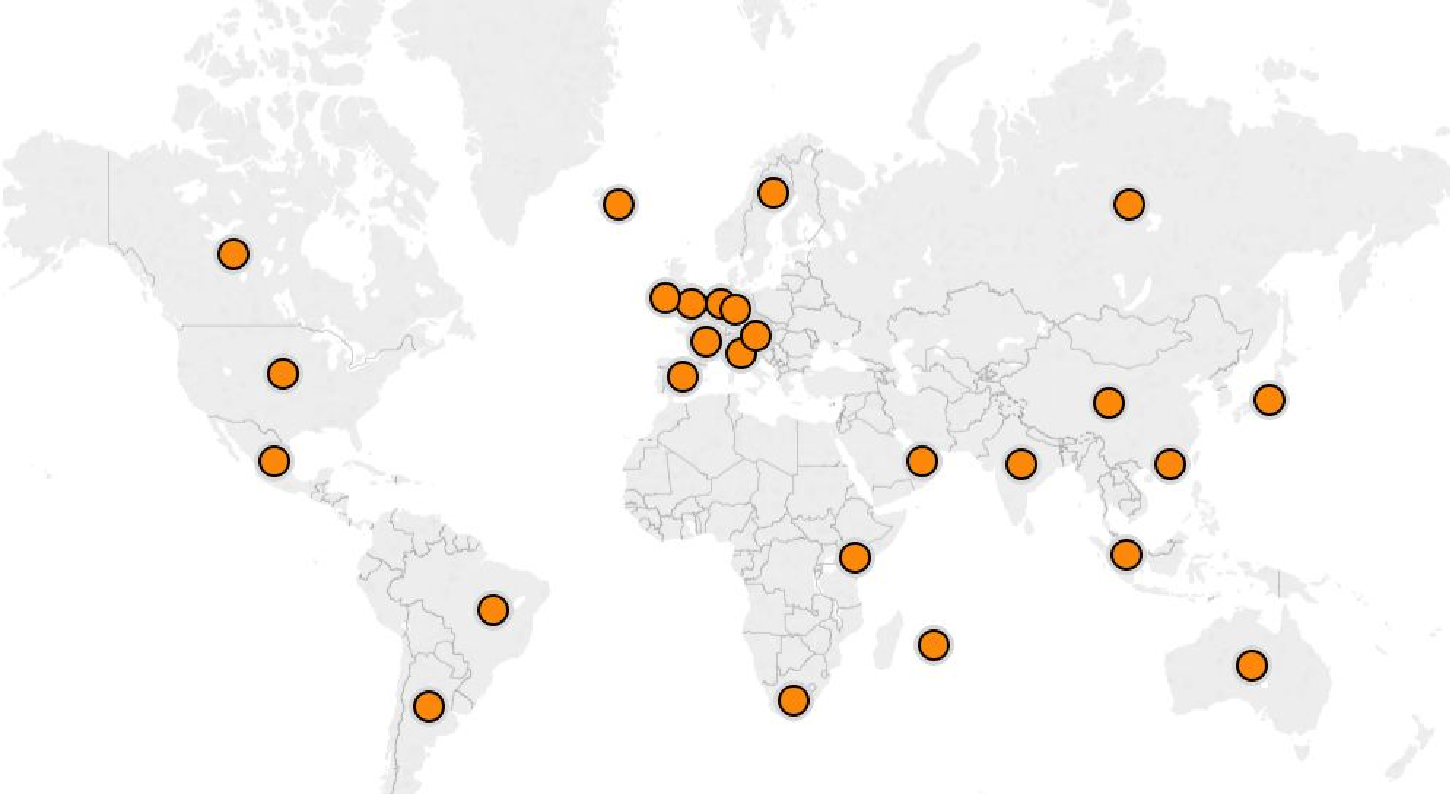
\includegraphics[width=\columnwidth]{World-DNS}
\caption{The locations of vantage points in measuring hosting diversity.}
\label{fig:world}
\end{figure}

\begin{figure}[t]
\centering
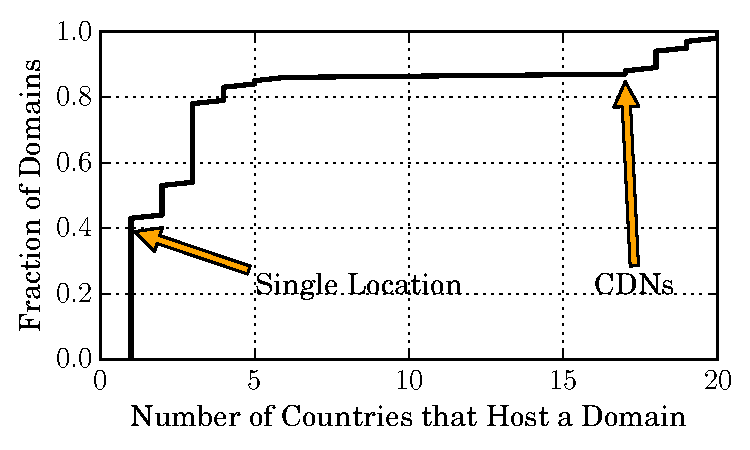
\includegraphics[width=\columnwidth]{domain_hist_US1}
\caption{The number of Alexa Top 100 US Domains hosted in different countries.}
\label{fig:host_diversity}
\end{figure}

\begin{finding}[Domain Hosting]
The most common destination among all five countries studied is the United States: 77\%, 45\%, 63\%, 44\%, and 97\% of paths originating in Brazil, Netherlands, India, Kenya and the United States, respectively, are currently reaching content located in the United States.
\end{finding}
The fraction of paths that are hosted in various countries can be seen in Table~\ref{tab:host}.  Despite the amount of country-level hosting diversity, we see the majority of paths from all five countries ending in a single country: the United States.  This is significant because the United States is a known surveillance state, and therefore these percentages represent the amount of foreign traffic that the United States can conduct surveillance on.  Our results also show the Netherlands is a common hosting location for traffic originating in the Netherlands, India, and Kenya.

%For Indian traffic, in addition to the 63\% hosted in the United States and the 10\% hosted in the Netherlands, another 10\% is hosted in Singapore.  Hosting in these countries can best be explained by the number of underwater cables with landing points in both India and Singapore~\cite{cablemap}.  More specifically, there is a cable that directly connects Chennai, India and Changi North, Singapore, and is owned by Tata Communications, which is one of the top global Internet providers (in terms of transitted IP space)~\cite{bakers}.  

%For Kenyan traffic, the United States hosts 44\% of the content, but Ireland hosts 10\%; Ireland is a popular hosting location for U.S. companies due to its relaxed enforcement of privacy in the private sector \annie{I got this information from Joel Reidenberg - how do I cite that?  I'll also look to see if I can find any publications that discuss this}.  

\begin{finding}[Domestic Traffic]
All of the countries studied (except for the United States) host content for a small percentage of their own traffic; they also host a small percentage of the their respective country code top-level domains.
\end{finding}
For traffic that originates in Brazil, only 17\% of it also ends in Brazil.  Only 5\% and 2\% of Indian and Kenyan traffic, respectively, end in the originating country. 
For Kenya, 24 of the Top 100 Domains are .ke domains, and of these 24 domains only 5 are hosted within Kenya.  29 out of 40 .nl domains are hosted in the Netherlands; 4 of 13 .in domains are hosted in India; 18 of 39 .br domains are hosted in Brazil.  Interestingly, all .gov domains were hosted in their respective country. 

\begin{finding}[Transit Traffic]
Surveillance states (specifically the United States and Great Britain) transit the largest portion of traffic in comparison to any other (foreign) country.
\end{finding}
Brazilian traffic traverses the United States on 84\% of the paths; therefore, the United States can conduct surveillance on 84\% of the traffic originating in Brazil, despite Brazil's strong efforts in avoiding United States surveillance.  Even though India and Kenya are geographically distant, 72\% and 62\% of their traffic transits the United States.   

Great Britain and the Netherlands are on the path for a significant percentage of traffic originating in India and Kenya.  50\% and 20\% of paths that originate in Kenya and India transit Great Britain.  Traffic that traverses the Netherlands can be explained by the large IXP located there; traffic that traverses Great Britain is likely due to being on the path between the originating country and the final destination in a European country.

Mauritius, South Africa, and the United Arab Emirates transit 32\%, 33\%, and 15\% of traffic from Kenya.  There are direct underwater cables from Kenya to Mauritius, and from Mauritius to South Africa~\cite{cablemap}.  Additionally, there is a cable from Mombasa, Kenya to Fujairah, United Arab Emirates.  This accounts for the large percentages of traffic that pass through these countries.

\begin{finding}[Tromboning Traffic]
Brazilian and Netherlands traffic often trombones to the United States, despite the prevalence of IXPs in both countries.
\end{finding}
As mentioned above, the percentage of domestic traffic in some of the countries studied is extremely small.  For India, only 5\% of traffic is domestic and for Kenya, 2\% is domestic; despite the small amount of domestic traffic, some of this traffic trombones.  This can be seen better in the cases of Brazil and the Netherlands; 
Figures \ref{fig:trombone_netherlands}, \ref{fig:trombone_brazil}, and \ref{fig:trombone_kenya} show the amount of paths that trombone to different countries for the Netherlands, Brazil, and Kenya. 24\% of all paths originating in the Netherlands (62\% of domestic traffic) trombone to a foreign country before returning to the Netherlands. Despite Brazil's strong efforts in building IXPs to keep local traffic local, we can see that their traffic still trombones to the United States.  This is due to IXPs being seen as a threat by competing commercial providers; providers are sometimes concerned that ``interconnection'' will result in making business cheaper for competitors and stealing of customers~\cite{ixp_policy}.  It is likely that Brazilian providers see other Brazilian providers as competitors and therefore as a threat at IXPs, which causes them to peer with international providers instead of other local providers.

\begin{figure*}[t!]
\begin{minipage}{\linewidth}
\begin{subfigure}[b]{.32\linewidth}
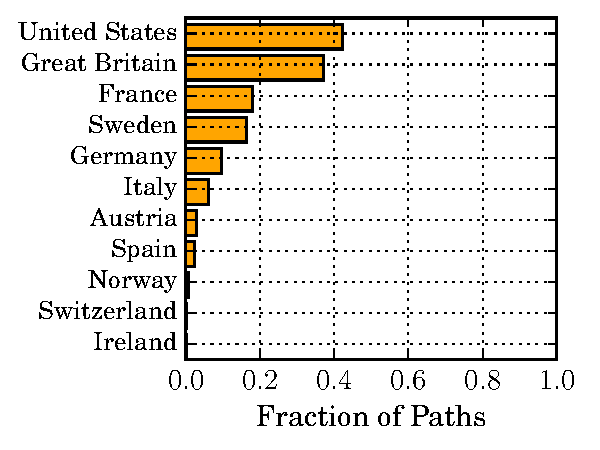
\includegraphics[width=\linewidth]{nl_trombone_new11}
\caption{The Netherlands.\label{fig:trombone_netherlands}}
\end{subfigure}\qquad
\begin{subfigure}[b]{.32\linewidth}
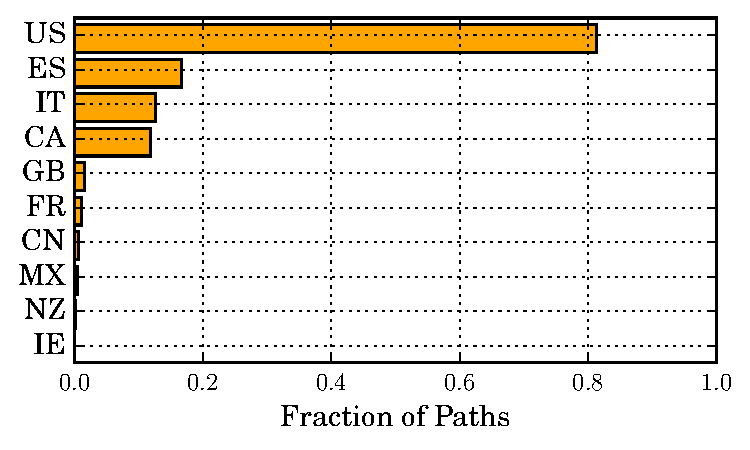
\includegraphics[width=\linewidth]{br_trombone_new11}
\caption{Brazil.\label{fig:trombone_brazil}}
\end{subfigure}\qquad
\begin{subfigure}[b]{.32\linewidth}
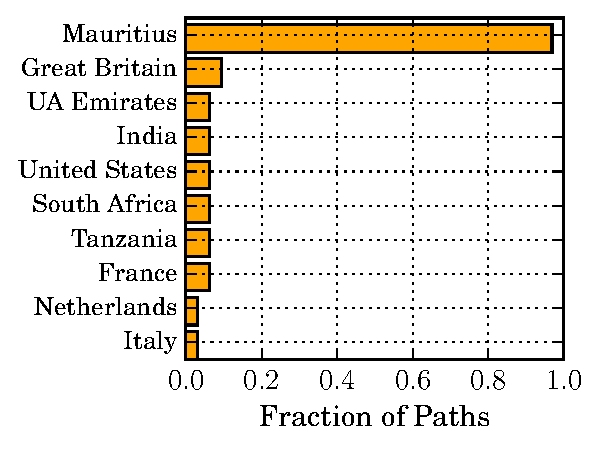
\includegraphics[width=\linewidth]{ke_trombone_new11}
\caption{Kenya.\label{fig:trombone_kenya}}
\end{subfigure}
\end{minipage}
\caption{The countries that tromboning traffic from the Netherlands, Brazil, and Kenya transits.}
\label{fig:trombone}
\end{figure*}

  %Traffic that should be kept local is susceptible to surveillance because it transits two well-known surveillance states.  

\begin{finding}[United States as an Outlier]
The United States hosts 97\% of the content that is accessed from within the country, and only 6 foreign countries---France, Germany, Ireland, Great Britain, and the Netherlands---- host content for the other 3\% of traffic.
\end{finding}
Most of the results discussed thus far have shown that Brazilian, Netherlands, Indian, and Kenyan traffic often transit surveillance states, most notably the United States.  The results from studying traffic that originates in the United States are drastically different from those of the other four countries.  The other four countries hosted very small amounts of their own traffic, whereas the United States hosts 97\% of the content that is accessed from within the country.  Only 13 unique countries are ever on a path from the United States to a domain in the top 100 (or third party domain), whereas 30, 30, 25, and 38 unique countries are seen on the paths originating in Brazil, Netherlands, India, and Kenya.  

%There are only 6 foreign countries---France, Germany, Ireland, Great Britain, and the Netherlands----that host content for traffic originating in the United States, and the fraction of content hosted in these countries is less than 4\% combined.

\subsection{Limitations}
The measurement methods that we described in Section~\ref{datasets} are not without limitations.  First, our study is solely based on IPv4 routes, which likely differ from IPv6 routes.  Here we also discuss limitations with IPv4, country mapping accuracy, and traceroute completeness.

\subsubsection{IPv4}
The measurements we conducted only collect and analyze IPv4 paths, and therefore all IPv6 paths are left out of our study.  IPv6 paths likely differ from IPv4 paths as not all routers that support IPv4 also support IPv6.  Future work includes studying IPv6 paths and which countries they transit, as well as a comparison of country avoidability between IPv4 and IPv6 paths. 

\subsubsection{Country Mapping}
Previous work has shown that there are fundamental challenges in deducing a geographic location from an IP address, despite using different methods such as DNS names of the target, network delay measurements, and host-to-location mapping in conjunction with BGP prefix information~\cite{padmanabhan2001investigation}.  While it has been shown that there are inaccuracies and incompleteness in MaxMind's data~\cite{huffaker2011geocompare}, the focus of this work is on measuring and avoiding surveillance, and not on geolocation algorithms, we therefore used a pre-existing geolocation service. Additionally, we discuss how we address inaccuracies and incompleteness in Section \ref{c_map}.

\subsubsection{Traceroute Accuracy and Completeness}
Our study is limited by the accuracy and completeness of traceroute.  Anomalies can occur in traceroute-based measurements~\cite{augustin2006avoiding}, but most traceroute anomalies do not cause an overestimation in surveillance states.  The incompleteness of traceroutes, where a router does not respond, causes our results to underestimate the number of surveillance states, and therefore also provides a lower bound on surveillance.

\section{Nation-State Routing: Default \\Routes}
\label{measure}

\newcommand{\headrow}[1]{\multicolumn{1}{c}{\adjustbox{angle=45,lap=\width-0.5em}{#1}}}
\newcolumntype{P}[1]{>{\raggedright\arraybackslash}p{#1}}
\begin{table*}[t]
\centering
\begin{tabular}{|P{37mm}|cc|cc|cc|cc|cc|}
\multicolumn{1}{l}{}    & \headrow{Host} & \headrow{Transit} & \headrow{Host} & \headrow{Transit} &\headrow{Host} &\headrow{Transit} &\headrow{Host}   &\headrow{Transit} &\headrow{Host}  &\headrow{Transit} \\\hline
\textit{Country}    &\multicolumn{2}{c|}{\textit{Brazil}}   &\multicolumn{2}{c|}{\textit{Netherlands}}   &\multicolumn{2}{c|}{\textit{India}} &\multicolumn{2}{c|}{\textit{Kenya}} &\multicolumn{2}{c|}{\textit{United States}}\\
\hline\hline
Brazil             &.169     &1.00   &     &  &   &   &    &     &  & \\\hline
Canada             &.001     &.013   &.007     &.007  &.015    &.016   &.006    &.008     &  &.081 \\\hline
France             &.001     &.059   &.022     &.102  &.009    &.104   &.023    &.221     &.0013  &.104 \\\hline
Germany             &.002     &.005   &.013     &.050  &.014    &.032   &.028    &.048     &.0013  &.008 \\\hline
Great Britain             &.00006     &.024   &.019     &.140  &.021    &.204   &.032    &.500     &.0024  &.006 \\\hline
India             &    &   &     &.0007  &.053   &1.0   &.002    &.058     &  &.0005 \\\hline
Ireland             &.016     &.028   &.064     &.106  &.027    &.031   &.108    &.133     &.0012  &.006 \\\hline
Kenya             &    &   &     &  &   &   &.022    &1.0     &  & \\\hline
Mauritius             &     &   &     &  &    &   &.004    &.322     &  & \\\hline
Netherlands             &.013     &.019   &.392     &1.0  &.101    &.121   &.200    &.253     &.024  &.031 \\\hline
Singapore             &    &.0009   &.002     &.002  &.103    &.270   &.027    &.040     &  &.003 \\\hline
South Africa             &    &   &     &  &   &   &.021    &.334     &  & \\\hline
Spain             &.001     &.176   &    &.004  &   &   &   &     &  & \\\hline
United Arab Emirates             &     &.00003   &     &  &   &   &.011    &.152     &  & \\\hline
United States             &.774     &.844   &.454     &.583  &.629    &.715   &.443    &.616     &.969  &1.0 \\\hline
\end{tabular}
\caption{Fraction of paths that each country sees in default routes.}
\label{tab:transit_host}
\end{table*}

As Internet traffic crosses international borders, it becomes subject to the wiretapping policies of the national jurisdiction in which it is transitting.  We study five different countries, Brazil, Netherlands, India, Kenya, and the United States, and measure which countries are transitting their traffic.  The methods we use are described in Section \ref{pipeline1}, and in this section we discuss our findings.

\subsection{Hosting Diversity}
First we look at hosting diversity.  This shows us how many unique countries in which a domain is hosted -- the more countries that a domain is hosted in creates a greater chance that the content is replicated in a favorable country, and could potentially allow a client to circumvent an unfavorable country.  By querying DNS from 26 vantage points around the world, we found that there is hosting diversity among the Alexa Top 100 Domains.  About half of the Alexa Top 100 Domains in each of the five countries studied are hosted in more than one country.  This can be seen in Figure~\ref{fig:host_diversity}.  The amount of hosting diversity motivates the potential for circumventing surveillance states.  We next look at which countries are currently transitting and hosting Internet traffic, and measure whether traffic is going to replicas in surveillance states (when they may not need to).

\begin{figure}
\centering
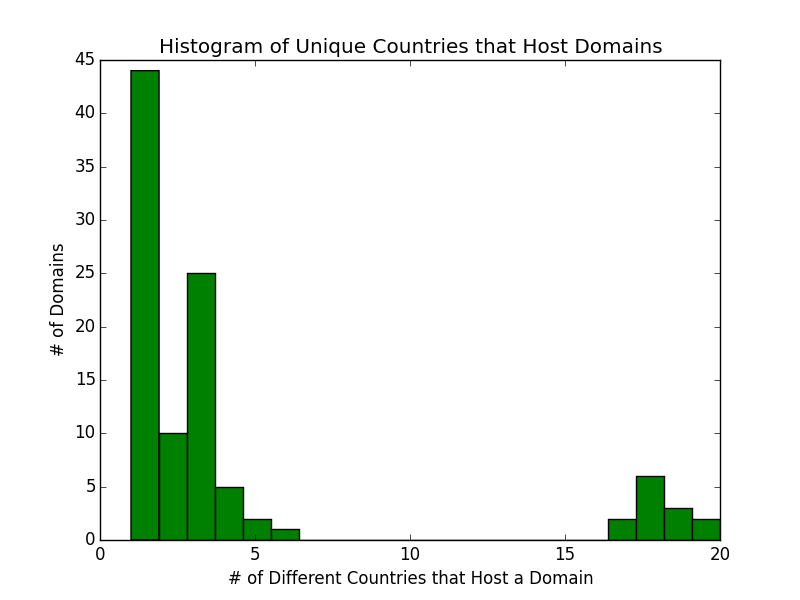
\includegraphics[width=.5\textwidth]{host_domains_hist_US}
\caption{The number of Alexa Top 100 US Domains hosted in different countries.}
\label{fig:host_diversity}
\end{figure}

\subsection{Trend 1: Surveillance States Host Domains}
\label{trend1}
Despite the amount of country-level hosting diversity, we see the majority of paths from all five countries ending in a single country.  The fraction of paths that are hosted in various countries can be seen in Table~\ref{tab:transit_host}.  The most common destination among all five countries studied is the United States: 77\%, 45\%, 63\%, 44\%, and 97\% of paths originating in Brazil, Netherlands, India, Kenya and the United States, respectively, are currently reaching content located in the United States.  This is significant because the United States is a known surveillance state, and therefore these percentages represent just a portion of foreign traffic that the United States can conduct surveillance on.  Our results also show the Netherlands as a common hosting location for traffic originating in the Netherlands, India, and Kenya.

For Indian traffic, in addition to the 63\% hosted in the United States and the 10\% hosted in the Netherlands, another 10\% is hosted in Singapore.  This can best be explained by the number of underwater cables with landing points in both India and Singapore~\cite{cablemap}.  More specifically, there is a cable that directly connects Chennai, India and Changi North, Singapore, and is owned by Tata Communications, which is one of the top global Internet providers (in terms of transitted IP space)~\cite{bakers}.  

For Kenyan traffic, the United States hosts 44\% of the content, but Ireland hosts 10\%; Ireland is a popular hosting location for U.S. companies due to it's relaxed enforcement of privacy in the private sector.  

It is also worth noting that most of the countries studied host a small percentage of their own traffic.  For traffic that originates in Brazil, only 17\% of it also ends in Brazil.  Only 5\% and 2\% of Indian and Kenyan traffic, respectively, end in the originating country.  In addition, only a fraction of country code top-level domains are hosted with in the respective country.  For Kenya, 24 of the Top 100 Domains are .ke domains, and of these 24 domains only 5 are hosted within Kenya.  29 out of 40 .nl domains are hosted in the Netherlands; 4 of 13 .in domains are hosted in India; 18 of 39 .br domains are hosted in Brazil.  Interestingly, all .gov domains were hosted in their respective country.

\subsection{Trend 2: Traffic Transits Surveillance States}
Similar to the trend of hosting domains, the United States also transits a large portion of foreign traffic -- it transits a larger portion of traffic than it hosts.  Brazilian traffic traverse the United States on 84\% of the paths; therefore, the United States can conduct surveillance on 84\% of the traffic originating in Brazil, despite Brazil's strong efforts in avoiding United States surveillance.  Even though India and Kenya are geographically distant, 72\% and 62\% of their traffic transits the United States.  Of the five countries studied, the Netherlands has the lowest percentage of traffic that transits the United States at 58\%.  

Great Britain and the Netherlands are on the path for a significant percentage of traffic originating in India and Kenya.  50\% and 20\% of paths that originate in Kenya and India transit Great Britain.  Traffic that traverses the Netherlands can be explained by the large IXP located there; traffic that traverses Great Britain is likely due to being on the path between the originating country and the final destination in a European country.

Mauritius, South Africa, and the United Arab Emirates transit 32\%, 33\%, and 15\% of traffic from Kenya.  There are direct underwater cables from Kenya to Mauritius, and from Mauritius to South Africa.  Additionally, there is a cable from Mombasa, Kenya to Fujairah, United Arab Emirates.  This accounts for the large percentages of traffic that pass through these countries.

\subsection{Trend 3: Tromboning Traffic Transits Surveillance States}

As mentioned in Section \ref{trend1}, the percentage of domestic traffic in some of the countries studied is extremely small.  For India, only 5\% of traffic is domestic and for Kenya, 2\% is domestic; despite the small amount of domestic traffic, some of this traffic trombones.  This can be seen better in the cases of Brazil and the Netherlands; figure \ref{trombone_netherlands} shows the amount of paths that trombone to differing countries for the Netherlands.

\begin{figure}
\centering
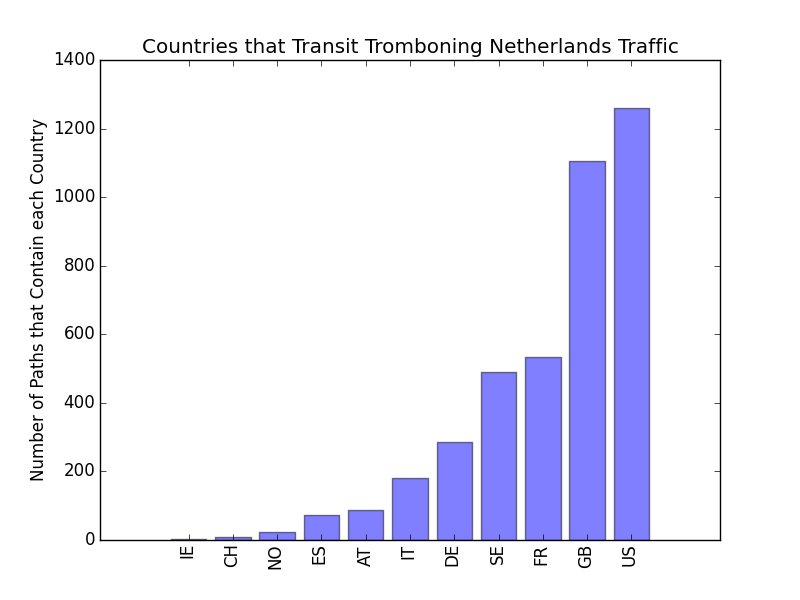
\includegraphics[width=.5\textwidth]{nl_trombone_no_none2}
\caption{The countries that tromboning Netherlands traffic transits.}
\label{fig:trombone_netherlands}
\end{figure}

24\% of all paths originating in the Netherlands (62\% of domestic traffic) trombone to a foreign country before returning to the Netherlands; The most common countries traffic trombones to are the United States and Great Britain.  Traffic that should be kept local is susceptible to surveillance because it transits two well-known surveillance states.  For Brazil, 5\% of all traffic starts in the Netherlands, transits a foreign country, and returns to the Netherlands (30\% of domestic traffic trombones).  The most common country traffic trombones to is the United States. 

\subsection{United States as an Outlier}

Most of the results discussed thus far have shown that Brazilian, Netherlands, Indian, and Kenyan traffic often transit surveillance states, most notable the United States.  The results from studying traffic that originates in the United States are drastically different from those of the other four countries.  The other four countries hosted very small amounts of their own traffic, whereas the United States hosts 97\% of the content that is accessed from witin the country.  Only 13 unique countries are ever on a path from the United States to a domain in the Top 100 (or third party domain), whereas 30, 30, 25, and 38 unique countries are seen on the paths originating in Brazil, Netherlands, India, and Kenya.  There are only 6 foreign countries that host content for traffic originating in the United States, and the fraction of content hosted in these countries is less than 4\% combined.

\section{Preventing Transnational Detours}
\label{avoid_results}
In light of the results from analyzing where \textit{current} traffic is going in Section \ref{datasets}, we evaluate the effectiveness of open resolvers and relays for country avoidance.  We discuss our measurement methods, introduce an avoidance metric and algorithm, and present our findings.

\subsection{Measurement Pipelines}

\paragraph{Country Avoidance with Open Resolvers.} If content is replicated in different parts of the world, open DNS resolvers located around the globe can potentially help clients circumvent surveillance states.  Our measurement pipeline is shown in Figure \ref{avoidance_resolvers}.  This measurement differs slightly from that described in Section \ref{pipeline}; instead of using RIPE Atlas probes to query local DNS resolvers, we query open DNS resolvers located around the world~\cite{open_resolver_list}.  These open DNS resolvers may provide different IP addresses in the DNS responses, which represent different locations of content replicas. The measurement study in Section \ref{pipeline} used RIPE Atlas probes to traceroute to the IP addresses in DNS response, but our measurement method here uses a VPN connection to the client's country, and then traceroutes (through the VPN connection) to the IP addresses in the DNS responses given by the open resolvers.  We use a VPN connection instead of RIPE Atlas probes because of the resource limitations discussed in Section \ref{resource_limits}; because this measurement would have cost more credits than we had, we used an alternative method that still represents an Internet user in each of the five countries studied.

\begin{figure}[t]
\centering
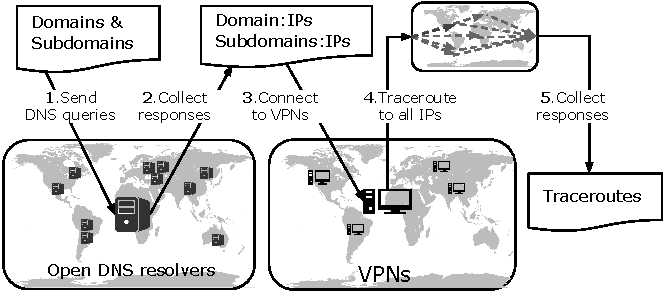
\includegraphics[width=.45\textwidth]{Country-Avoidance-Resolvers}
\caption{Measurement pipeline for country avoidance with open DNS resolvers.}
\label{fig:avoidance_resolvers}
\end{figure}

\paragraph{Country Avoidance with Relays.} Using an overlay network may help clients route around unfavorable countries or access content that is hosted in a more favorable country.  Figure \ref{fig:avoidance_relays} shows the steps to conduct this measurement.  After selecting relay machines, we run traceroute measurements from Country X to each relay and from each relay to the set of domains. 

\begin{figure}[t]
\centering
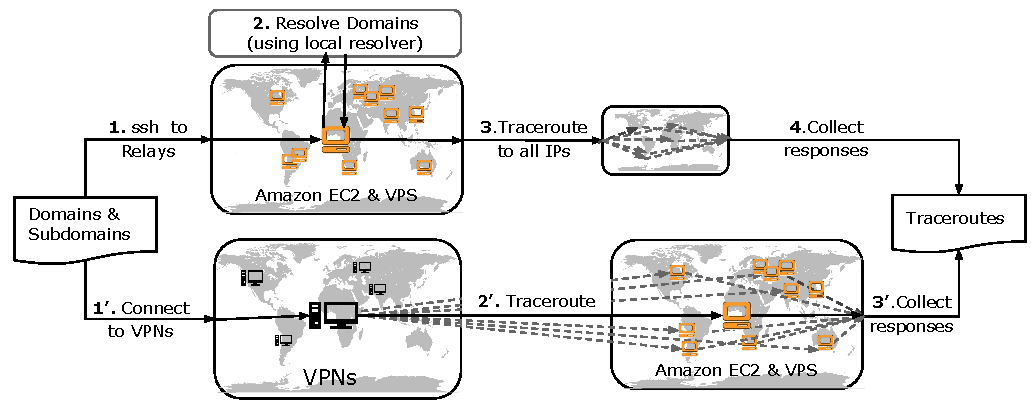
\includegraphics[width=.55\textwidth]{Country-Avoidance-Relays}
\caption{Measurement pipeline for country avoidance with overlay network relays.}
\label{fig:avoidance_relays}
\end{figure}

We use eight Amazon EC2 instances, one in each geographic region (United States, Ireland, Germany, Singapore, South Korea, Japan, Australia, Brazil), as well as 4 VPS (Virtual Private Server) machines (France, Spain, Brazil, Singapore), which are virtual machines that are functionally equivalent to dedicated physical servers.  The conjunction of these two sets of machines allow us to evaluate surveillance avoidance with a geographically diverse set of relays. By selecting an open resolver in each country that also has a relay in it we can keep the variation in measurement methods low, leading to a more accurate comparison of country avoidance methods.

\subsection{Avoidability Metrics}
\label{metrics}
We introduce a new metric and algorithm to measure how often a client in Country X can avoid a specific Country Y.  Using the proposed metric and algorithm, we can compare how well the different methods achieve country avoidance for any (Country X, Country Y) pair.

\paragraph{Avoidability Metric.}  This metric quantifies how often traffic can avoid Country Y when it originates in Country X.  Avoidability is explained as the fraction of paths that start in Country X and do not transit Country Y; more formally:

\[Avoidability(X,Y) = \frac{paths_{X,\bcancel{Y}}}{paths_{X}}\]

\noindent where $paths_{X,\bcancel{Y}}$ represent the paths from Country X that do not pass through Country Y, and $paths_{X}$ represent all paths that originate from Country X. The resulting value will be in the range [0,1], where 0 means the country is unavoidable for all of the domains in our study, and 1 means the client can avoid Country Y for all domains in our study.  We use this metric on country-level paths, as described in Section~\ref{pipeline}.

\paragraph{Avoidability Algorithm with Relays.}  Measuring the avoidability of a country Y from a client in Country X using relays has two components: 1) is Country Y on the path from the client in Country X to the relay?  2) is Country Y on the path from the relay to the domain?  For every domain, our algorithm checks if there exists at least one path from the client Country X through any relay and on to the domain, and does not transit Country Y.  The psuedo-code for the algorithm is shown in Algorithm~\ref{avoid_algo}.

\begin{algorithm}[t]
\caption{Avoidability Algorithm}
\label{avoid_algo}
\begin{algorithmic}[1]
\Function{CalcAvoidance}{set $paths1$, set $paths2$, string c}
    \State set $usableRelays$
    \For{each $(relay,path)$ in $paths1$} 
    	\If{$c$ not in $path$}
		\State $usableRelays \gets path$
	\EndIf
    \EndFor
    \State set $accessibleDomains$
    \For{each $(relay,domain,path$ in $paths2$}
    \If{$relay$ in $usableRelays$}
        \If{$c$ not in $path$}
        \State $accessibleDomains \gets domain$
        \EndIf
    \EndIf
    \EndFor
    \State $D \gets$ number of all unique domains in $paths2$
    \State $A \gets$ length of $accessibleDomains$
    \State \Return $A / D$
\EndFunction
\end{algorithmic}
\end{algorithm}

The output of the algorithm is a value in the range [0,1] that can be compared to the output of the Avoidability Metric described above.  

\paragraph{Upper bound on Avoidability.}  While the Avoidability metric and algorithm provide a method to quantify how avoidable Country Y is from a client in Country X, it may be the case that a number of domains are hosted in Country Y, so the Avoidance value for these countries would never reach 1.0.  For this reason, we measured the upper bound on avoidance for given pair of (Country X, Country Y) that represents the best case value for avoidance.  The pseudocode for the algorithm is shown in Algorithm \ref{upperbound_algo}.

\begin{algorithm}[t]
\caption{Avoidance Upper bound Algorithm}
\label{upperbound_algo}
\begin{algorithmic}[1]
\Function{CalcUpperbound}{set $relayDomainPaths$, string $c$}
    \State $zeros(domainLocations)$
    \For{each $(r,d,p)$ in $relayDomainPaths$} 
		\State $dest \gets $ last item in $p$
		\State $domainLocations[d] \gets dest$
    \EndFor
    \State set $accessibleDomains$
    \For{each $domain$ in $domainLocations$}
    \If{$domainLocations[domain] \neq $ set[$c$]}
    \State $accessibleDomains \gets domain$
    \EndIf
    \EndFor
    \State $D \gets$ all unique domains in  $relayDomainPaths$
    \State $A \gets$ length of $accessibleDomains$
    \State \Return $A / D$
\EndFunction
\end{algorithmic}
\end{algorithm}

The algorithm analyzes the destinations of all domains from all relays and if there exists at least one destination for a domain that is not in Country Y, then this increases the upper bound value.  An upper bound value of 1.0 means that every domain studied is hosted (or has a replica) outside of Country Y.  This value puts the Avoidance values in perspective for each (Country X, Country Y) pair. 

\subsection{Results}
After applying the metrics described in Section \ref{metrics} to country-level paths, we compared avoidance values when using open resolvers, when using relays, and when using no country avoidance tool.  First, we discuss how effective open resolvers are at country avoidance.  Then we show how effective relays are at country avoidance as well as at keeping local traffic local.  Avoidance values are shown in Table \ref{tab:avoid}, where the countries we studied are shown in the top row, and the country to avoid is in the left-most column.  

\newcolumntype{d}[1]{D{.}{.}{#1}}
\begin{table*}[t]
\centering
\begin{tabular}{P{32mm}|d{3.2}d{3.2}|d{3.2}d{3.2}|d{3.2}d{3.2}|d{3.2}d{3.2}|d{3.2}d{3.2}}
\multicolumn{1}{l}{}    & \headrow{No Relay} & \headrow{Relays} & \headrow{No Relay} & \headrow{Relays} & \headrow{No Relay} & \headrow{Relays}   & \headrow{No Relay} & \headrow{Relays}  & \headrow{No Relay} & \headrow{Relays} \\ \toprule
\textit{Country}    &\multicolumn{2}{c|}{\textit{Brazil}}   &\multicolumn{2}{c|}{\textit{Netherlands}}   &\multicolumn{2}{c|}{\textit{India}} &\multicolumn{2}{c|}{\textit{Kenya}} &\multicolumn{2}{c}{\textit{United States}}\\ \toprule

Brazil               &0.00     &0.00     &1.00  &1.00   &1.00    &1.00  &1.00   &1.00  &1.00  &1.00  \\ \midrule
Canada               &.98     &1.00     &.99  &1.00   &.98    &.98  &.99   &.99  &.92  &1.00  \\
United States        &\cellcolor[HTML]{F7BE81}.15     &\cellcolor[HTML]{F7BE81}.62     &\cellcolor[HTML]{F7BE81}.41  &\cellcolor[HTML]{F7BE81}.63   &\cellcolor[HTML]{F7BE81}.28    &\cellcolor[HTML]{F7BE81}.65  &\cellcolor[HTML]{F7BE81}.38   &\cellcolor[HTML]{F7BE81}.40  &\cellcolor[HTML]{F7BE81}0.00  &\cellcolor[HTML]{F7BE81}0.00  \\ \midrule
France               &.94     &1.00     &.89  &.99   &.89    &1.00  &.77   &.98  &.89  &.99  \\
Germany              &.99     &1.00     &.95  &.99   &.96    &.99  &.95   &1.00  &.99  &1.00  \\
Great Britain        &.97     &1.00     &.86  &.99   &\cellcolor[HTML]{F7BE81}.79    &\cellcolor[HTML]{F7BE81}1.00  &\cellcolor[HTML]{F7BE81}.50   &\cellcolor[HTML]{F7BE81}.97  &.99  &1.00  \\
Ireland              &.97     &.99     &.89  &.99   &.96    &.99  &.86   &.99  &.99  &.99  \\
Netherlands          &.98     &.99     &0.00  &0.00   &.87    &.99  &\cellcolor[HTML]{F7BE81}.74   &\cellcolor[HTML]{F7BE81}.99  &.97  &.99  \\
Spain                &.82     &1.00     &.99  &.99   &1.00    &1.00  &1.00   &1.00  &1.00  &1.00  \\ \midrule
Kenya                &1.00     &1.00     &1.00  &1.00   &1.00    &1.00  &0.00   &0.00  &1.00  &1.00  \\
Mauritius            &1.00     &1.00     &1.00  &1.00   &1.00    &1.00  &\cellcolor[HTML]{F7BE81}.67   &\cellcolor[HTML]{F7BE81}.99  &1.00  &1.00  \\
South Africa         &1.00     &1.00     &1.00  &1.00   &1.00    &1.00  &\cellcolor[HTML]{F7BE81}.66   &\cellcolor[HTML]{F7BE81}.66  &1.00  &1.00  \\ \midrule
United Arab Emirates &1.00     &1.00     &1.00  &1.00   &1.00    &1.00  &.84   &.99  &1.00  &1.00  \\
India                &1.00     &1.00     &.99  &1.00   &0.00    &0.00  &.94   &1.00  &.99  &1.00  \\
Singapore            &.99     &1.00     &.99  &1.00   &\cellcolor[HTML]{F7BE81}.73    &\cellcolor[HTML]{F7BE81}.94  &.96   &1.00  &.99  &1.00  \\\midrule
\end{tabular}
\caption{Avoidance values for different techniques of country avoidance.  The upper bound on avoidance is 1.0 in most cases, but not all.  It is 
common for some European countries to host a domain, and therefore the upper bound is slightly lower than 1.0.  The upper bound on avoidance of the 
United States is significantly lower than the upper bound on avoidance for any other country; .886, .790, .844, and .765 are the upper bounds on avoidance 
of the United States for traffic originating in Brazil, Netherlands, India, and Kenya, respectively.}
\label{tab:avoid}
\end{table*}

\subsubsection{Avoidance with Open Resolvers}
\annie{This is still being calculated, but I'll update as soon as possible.}

\subsubsection{Avoidance with Relays}
As seen in Table \ref{tab:avoid}, there are two significant trends: 1) the ability for a client to avoid a given Country Y increases with the use of relays, and 2) the least avoidable countries are surveillance states.

\begin{finding}[Relay Effectiveness]
For 84\% of the (Country X, Country Y) pairs shown in Table \ref{tab:avoid} the avoidance with relays reaches the upper bound on avoidance. 
\end{finding}
In almost every (Country X, Country Y) pair, where Country X is the client's country (Brazil, Netherlands, India, Kenya, or the United States) and Country Y is the country to avoid, the use of an overlay network makes Country Y more avoidable than the current default routes.  The one exception we encountered is when a client is located in Kenya and wants to avoid South Africa; South Africa is on the path between the client and every relay, and therefore the client should not use the relays.  

\begin{finding}[Relays Achieve Upper Bound]
For clients in the United States, 100\% of avoidance values reach the upper bound---relays help clients in this country avoid all other Country Y in all cases that the domain is not hosted in Country Y.  
\end{finding}
Relays are most effective for clients in the United States.  On the other hand, (Kenya, Country Y) pairs have the lowest percentage of avoidance values that reach the upper bound, showing that it is more difficult for Kenyan clients to avoid a given country.  This is not to say that relays are not effective for clients in Kenya; for example, the default routes to the top 100 domains for Kenyans avoid Great Britain 50\% of the time, but with relays this percentage increases to about 98\% of the time, and the upper bound is about 98\%. 
%Figure \ref{fig:ke_avoidance} shows default avoidance, avoidance with relays, and the upper bound for Kenya; it's clear that despite having the worst position for avoidance out of the studied countries, in most cases the avoidance with relays either reaches or because extremely close to the upper bound.  

\begin{finding}[Surveillance States are Less Avoidable]
Avoidance values for (Country X, United States) pairs are significantly lower than any other Country Y for all three situations: without relays, with relays, and the upper bound. 
\end{finding}
%Certain surveillance states discussed in Section \ref{surv} are completely unavoidable a small fraction of time from certain client locations.  France is unavoidable for a small percentage of domains for clients located in the Netherlands, Kenya, and the United States.  Similarly, clients in the Netherlands and Kenya cannot avoid Great Britain for a small fraction of domains.  

Despite increasing clients' ability to avoid the United States, relays are not as effective at helping clients avoid this country as compared to the effectiveness of the relays at avoiding all other Country Y.  Clients in India can avoid the United States more often than clients in Brazil, Netherlands, and Kenya, with an avoidance value of .656 when using relays.  Kenyan clients can only avoid the United States 40\% of the time even while using relays.  Additionally, the upper bound for avoiding the United States is significantly lower in comparison to any other country.  

\begin{finding}[Local Traffic]
Using relays, the percentage of tromboning traffic decreased, and the number of countries that traffic tromboned to decreased.
\end{finding}
For the cases where there were relays located in one of the five studied countries, we evaluated how effectively the use of relays kept local traffic local.  This evaluation was possible for Brazil and the United States.  Tromboning Brazilian traffic decreased from 13.2\% without relays to 9.7\% with relays; when relays are used, all tromboning traffic goes only to the United States.  With the use of relays, there was only 1.3\% tromboning traffic for a United States client, whereas without relays there was 11.2\% tromboning traffic.  For the 1.2\% of traffic that trombones from the United States, it goes only to Ireland.

\section{Discussion}

\subsection{Why existing tools don't work}

\subsection{Alibi Routing}

\subsection{Security - Other Attackers}

\section{Related Work}
\label{related}

\paragraph{Nation-state routing analysis.}  Shah and
Papadopoulos recently measured international routing detours---paths that originate
in
one country, cross international borders, and then return to the
original country)---using public Border Gateway Protocol~(BGP) routing tables~\cite
{shah2015characterizing}. 
The study discovered 2 million detours each month out
of 7 billion total paths); the study also characterized the detours based
on detour dynamics and persistence.  Our work differs because it {\em actively}
measures traceroutes, yielding a more precise measurement of the path traffic is
likely to take, as opposed to analyzing BGP
routes.  Obar and Clement analyzed traceroutes
that started and ended in Canada, but tromboned through the United
States, and argued that
this is a violation of Canadian network
sovereignty~\cite{obar2012internet}. 
Karlin \ea developed a framework for country-level
routing analysis to study how much influence each country has over
interdomain routing~\cite{karlin2009nation}.  This work measures the
centrality of a country using BGP routes and AS-path inference; in contrast, our work uses active 
measurements and measures avoidability of a given country. 

\paragraph{Mapping national Internet topologies.}  Roberts \ea developed a method
for mapping national networks of ASes, identifying ASes that act as points of
control~\cite{roberts2011mapping}.   %JEN: not clear we care about the
"complexity" (whatever that means) %, and measuring the complexity of the
national network Several studies have also characterized network paths {\em
within} a country, including
Germany~\cite{wahlisch2010framework,wahlisch2012exposing} and
China~\cite{zhou2007chinese}, or a country's interconnectivity within a region
or with the rest of the
world~\cite{bischof2015and,gupta2014peering,fanou2015diversity}; these studies
focus on paths within a country of interest, as opposed to focusing on
transnational Internet paths.

\paragraph{Routing overlays and Internet architectures.} Alibi Routing uses
round-trip times to prove that that a client's packets did  not traverse a
forbidden country or region~\cite{levin2015alibi}; our work differs by
measuring  which countries a client's packets would (and does) traverse.  Our
work then  uses active measurements to determine the best path for a client
wishing  to connect to a server.  RON, Resilient Overlay Network, is an
overlay network that  routes around failures, whereas our overlay network
routes around countries~\cite{andersen2001resilient}.  ARROW introduces a
model that allows users to route around ISPs~\cite{peter2015one}, but requires
ISP participation, making it considerably more difficult to deploy than
\system{}. ARROW also aims to improve fault-tolerance, robustness, and
security, rather than explicitly attempting to avoid certain countries; ARROW
provides mechanisms to avoid individual ISPs, but such a mechanism is at a
different level of granularity, because an ISP may span multiple countries.
Zhang \ea presented SCION, a ``clean-slate'' Internet architecture that
provides route control, failure isolation, and explicit trust information for
communication~\cite{zhang2011scion}; SCION, however, requires fundamental
changes to the Internet architecture, whereas \system{} is deployable today.


\paragraph{Circumvention systems.}  Certain tools, such as anonymous
communications systems or virtual private networks, may use a combination of
encryption and overlay routing to allow clients to avoid surveillance. Tor is
an anonymity system that uses three relays and layered encryption to allow
users to communicate anonymously~\cite{dingledine2004tor}.  In contrast,
\system{} does not aim to achieve anonymity; instead, its aim is to ensure
that traffic does not traverse a specific  country, a goal that Tor cannot
achieve.  Even tools like Tor do not inherently thwart surveillance: Tor is
vulnerable to traffic correlation attacks and some attacks are possible even
on encrypted user traffic. VPNGate is a public VPN relay system aimed at
circumventing national firewalls~\cite{nobori2014vpn}. Unfortunately, VPNGate
does not allow a client to choose any available VPN, which makes it more
difficult for a user to ensure that traffic avoids a particular part of the
Internet.  Neither of these systems explicitly avoid countries; thus, they may
not  be able to avoid surveillance or the laws or jurisdiction of a particular
country. Additionally, existing circumvention systems generally rely on
encryption, which does not prevent surveillance; prior research has shown that
websites can be fingerprinted based on size, content, and location of third
party resources, which  reveals information about the content a user is
accessing \cite{what_isps_can_see}.  Finally, ISPs often execute man-in- the-
middle attacks on TLS connections to perform network management
functions~\cite{mitm_isp}.


\section{Conclusion}
\label{conclusion}

We have characterized routing
detours that take Internet paths through foreign countries, showing 
that underserved regions often depend on the United States and Europe to 
access popular content; this can cause performance degradation, increased costs, 
and gives more power to these dominant countries to perform surveillance and censorship.   %we have
%investigated how clients, ISPs, and governments can use overlay network relays to prevent routing detours through
%a given country.  This method gives clients the power to
%avoid certain countries, as well as help keep local traffic local.
%Although some countries are completely avoidable, we find that some of
%the more prominent surveillance states are the least avoidable.
As a first step towards a remedy, we have
designed, implemented, and deployed \system{}, which employs overlay network
relays to  route traffic around a given country; our data and code is publicly available~\cite{ransom_data,ran_system}.  %Our evaluation
%shows  that \system{} can in many cases avoid certain countries while
%performing nearly as well, if not better, than taking default routes.

%Our work presents several opportunities for follow-up studies and
%future work. First, Internet paths continually
%evolve; we will repeat this analysis over time and publish the results
%and data on a public website, to help deepen our collective
%understanding about how the evolution of Internet connectivity affects
%transnational routes. Second, our analysis should be extended to study
%the extent to which citizens in one country can avoid groups of
%countries or even entire regions. Finally, although our results provide strong 
%evidence for the existence of various transnational data flows, factors
%such as uncertain IP geolocation make it difficult to provide clients
%guarantees about country-level avoidance; developing techniques and
%systems that offer clients stronger guarantees
%is a ripe opportunity for future work.

%\end{document}  % This is where a 'short' article might terminate

%ACKNOWLEDGMENTS are optional
%\section{Acknowledgments}

%
% The following two commands are all you need in the
% initial runs of your .tex file to
% produce the bibliography for the citations in your paper.
\bibliographystyle{abbrv}
\bibliography{sigproc}  % sigproc.bib is the name of the Bibliography in this case
% You must have a proper ".bib" file
%  and remember to run:
% latex bibtex latex latex
% to resolve all references
%
% ACM needs 'a single self-contained file'!
%
%APPENDICES are optional
%\balancecolumns
%\appendix
%Appendix A
\end{document}
